\chapter{Introduction}

Encrypted ClientHello (ECH) is an emerging extension to the TLS 1.3 protocol which aims to protect sensitive metadata during the TLS handshake. While TLS encrypts application data, the initial ClientHello message remains unencrypted, revealing information such as the Server Name Indication (SNI) and Application-Layer Protocol Negotiation (ALPN). This information being shown in plain-text allows bad actors to monitor, profile, censor, or intercept users, even when TLS encryption is otherwise secure. ECH encrypts the ClientHelloInner message using Hybrid Public Key Encryption (HPKE) which conceals the intended domain and strengthens privacy at the network layer.

Lighttpd is a lightweight and high-performance open-source web server designed for environments where efficiency, low memory usage, and simplicity are essential. Unlike larger server platforms such as Apache or Nginx, Lighttpd prioritises a minimal footprint while maintaining support for modern web standards and extensible features through its modular architecture. Its event-driven design allows it to handle large volumes of concurrent connections with reduced overhead, making it suitable for embedded systems, resource-constrained deployments, and experimental research setups.

As ECH is relatively new and still undergoing standardisation, ECH is poorly tested. This project focuses on building a test environment. For ECH using a web server built with Lighttpd. The tests will include ......

\section{Motivation}

Metadata leakage remains a critical weakness even when content is fully encrypted. The SNI field in TLS has become a significant point of exposure, enabling censorship regimes, tracking systems, and other bad actors to monitor user activity. For organisations committed to user privacy including civil society groups, investigative journalists, and human rights organisations mitigating SNI-based surveillance is essential.

ECH offers a promising defence, but its deployment is not straightforward. Its reliance on experimental TLS libraries, DNS infrastructure, and non-standardised tooling creates high barriers for developers and researchers. There is also limited publicly available guidance documenting how ECH-enabled servers should be built, configured, and tested.

The motivation for this project is therefore twofold:
\begin{itemize}
    \item To create a reproducible ECH testing environment suitable for experimentation, debugging, and educational use.
    \item To evaluate Lighttpd's experimental ECH implementation, documenting its behaviour, limitations, and compatibility with BoringSSL's tooling.
\end{itemize}

A reliable ECH test harness lowers the barrier to future deployment, facilitates research into evolving protocol behaviour, and supports wider adoption.

\section{Project Objectives}

The central research question guiding this work is:

\begin{quote}
\emph{How can Encrypted ClientHello be enabled, tested, and validated on a Lighttpd web server in an effiecient reproducable manner?}
\end{quote}

This question is explored through the following objectives:

\begin{itemize}
    \item \textbf{Understand the ECH protocol and surrounding technologies.}  
    This involves studying TLS 1.3, HPKE, DNS integration requirements, and the structure of the ClientHelloInner and ClientHelloOuter messages. Practical experiments with BoringSSL are used to deepen understanding.

    \item \textbf{Compile and configure Lighttpd with ECH support.}  
    Lighttpd must be rebuilt from source and linked against BoringSSL. This includes modifying build flags, resolving dependency issues, and integrating ECH key material into the server configuration.

    \item \textbf{Develop an automated ECH test harness.}  
    Initial testing uses the \texttt{bssl client} debugging tool to inspect handshake behaviour. Later work incorporates automated browser-based testing with Playwright to simulate realistic client interactions.

    \item \textbf{Analyse behaviour through logged TLS handshakes.}  
    Focus is placed on interpreting negotiation states, debugging errors such as \texttt{TLSV1\_ALERT\_ECH\_REQUIRED}, and determining whether the server accepts, rejects, or attempts ECH negotiation under various configurations.

    \item \textbf{Incorporate automated browser-based testing.} Playwright and headless browsers are used to simulate realistic client behaviour, validate ECH negotiation in full browser stacks, and provide reproducible interaction traces for analysis.

\end{itemize}

These objectives establish the technical foundation for the implementation and analysis conducted throughout the project.

A biweekly timeline is shown below  fig 1.2.1
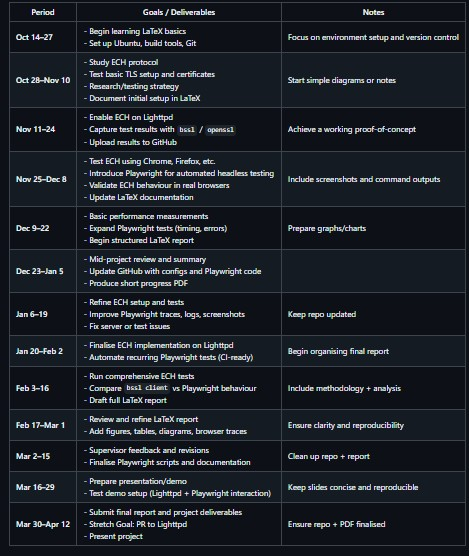
\includegraphics[width=\textwidth]{biweekly_timeline.jpg}

\section{Research Contributions}

This work makes the following contributions:

\begin{itemize}
    \item \textbf{A reproducible environment for building and testing ECH on Lighttpd.}  
    This includes the full toolchain for compiling BoringSSL, integrating it with Lighttpd, and generating ECH key material.

    \item \textbf{A detailed examination of ECH handshake behaviour.}  
    The project documents negotiation states, error modes, and observable behaviours such as \texttt{ECH\_REJECTED} that arise during experimental testing.

    \item \textbf{Analysis of Lighttpd's experimental ECH implementation.}  
    This includes identifying limitations, configuration pitfalls, and mismatches between BoringSSL's ECH formats and Lighttpd's expectations.

    \item \textbf{Platwright and headless browser.}  
    The project establishes tets using playwright and headless browser

\end{itemize}

The methodology developed here supports future researchers studying ECH adoption, debugging server implementations, and building larger interoperability test suites.



